% =====================================================================
\chapter{GIỚI THIỆU ĐỀ TÀI}\label{chap:gioithieu}
% =====================================================================

\section{Đặt vấn đề}
Tại các đô thị lớn, số lượng ô tô tăng nhanh hơn nhiều so với diện tích bãi đỗ. Người lái
thường phải đi vòng để tìm chỗ trống, gây ùn tắc cục bộ và lãng phí nhiên liệu. Ở các bãi
quy mô nhỏ như bãi của chung cư mini, văn phòng hay trường học, việc vận hành phần lớn vẫn
thủ công: vé giấy, ghi giờ bằng tay, tính tiền theo ước lượng của người trông xe và hầu như
không có cơ chế cảnh báo khi xảy ra cháy hoặc ngập nước, hai rủi ro thường gặp ở tầng hầm.

Từ thực trạng trên, đề tài đặt ra bài toán: với linh kiện phổ thông giá rẻ, xây dựng một hệ
thống tự động hóa trọn vẹn quy trình của một bãi xe nhỏ, từ lúc xe vào cổng, đỗ vào ô, cho
tới lúc thanh toán và rời bãi, đồng thời bảo đảm an toàn cho bãi trong suốt thời gian đó.
Bài toán này cũng là một ứng dụng điển hình của môn học, đòi hỏi lập trình đa tác vụ trên
hệ điều hành thời gian thực, điều khiển ngoại vi bằng phần cứng chuyên dụng và giao tiếp
không dây giữa nhiều vi điều khiển.

\section{Tổng quan về hệ thống}\label{sec:tongquan}
Hệ thống được hiện thực trên một mô hình bãi xe gồm 5 ô đỗ và hai cổng vào, ra có thanh
chắn. Hình~\ref{fig:overview} là ảnh chụp mô hình hoàn thiện nhìn từ trên xuống. Dãy ô đỗ
nằm dọc vách sau, mỗi ô có một cảm biến hồng ngoại xác định ô đó có xe hay không. Hộp điều
khiển ở giữa bãi chứa vi điều khiển trung tâm, màn hình hiển thị quay ra phía người lái và
hai đầu đọc thẻ RFID gắn ở hai bên hông, mỗi đầu đọc phục vụ một làn. Hai động cơ servo ở hai
góc trước nâng hạ thanh chắn của cổng vào (bên trái) và cổng ra (bên phải).

\begin{figure}[!t]
\centering
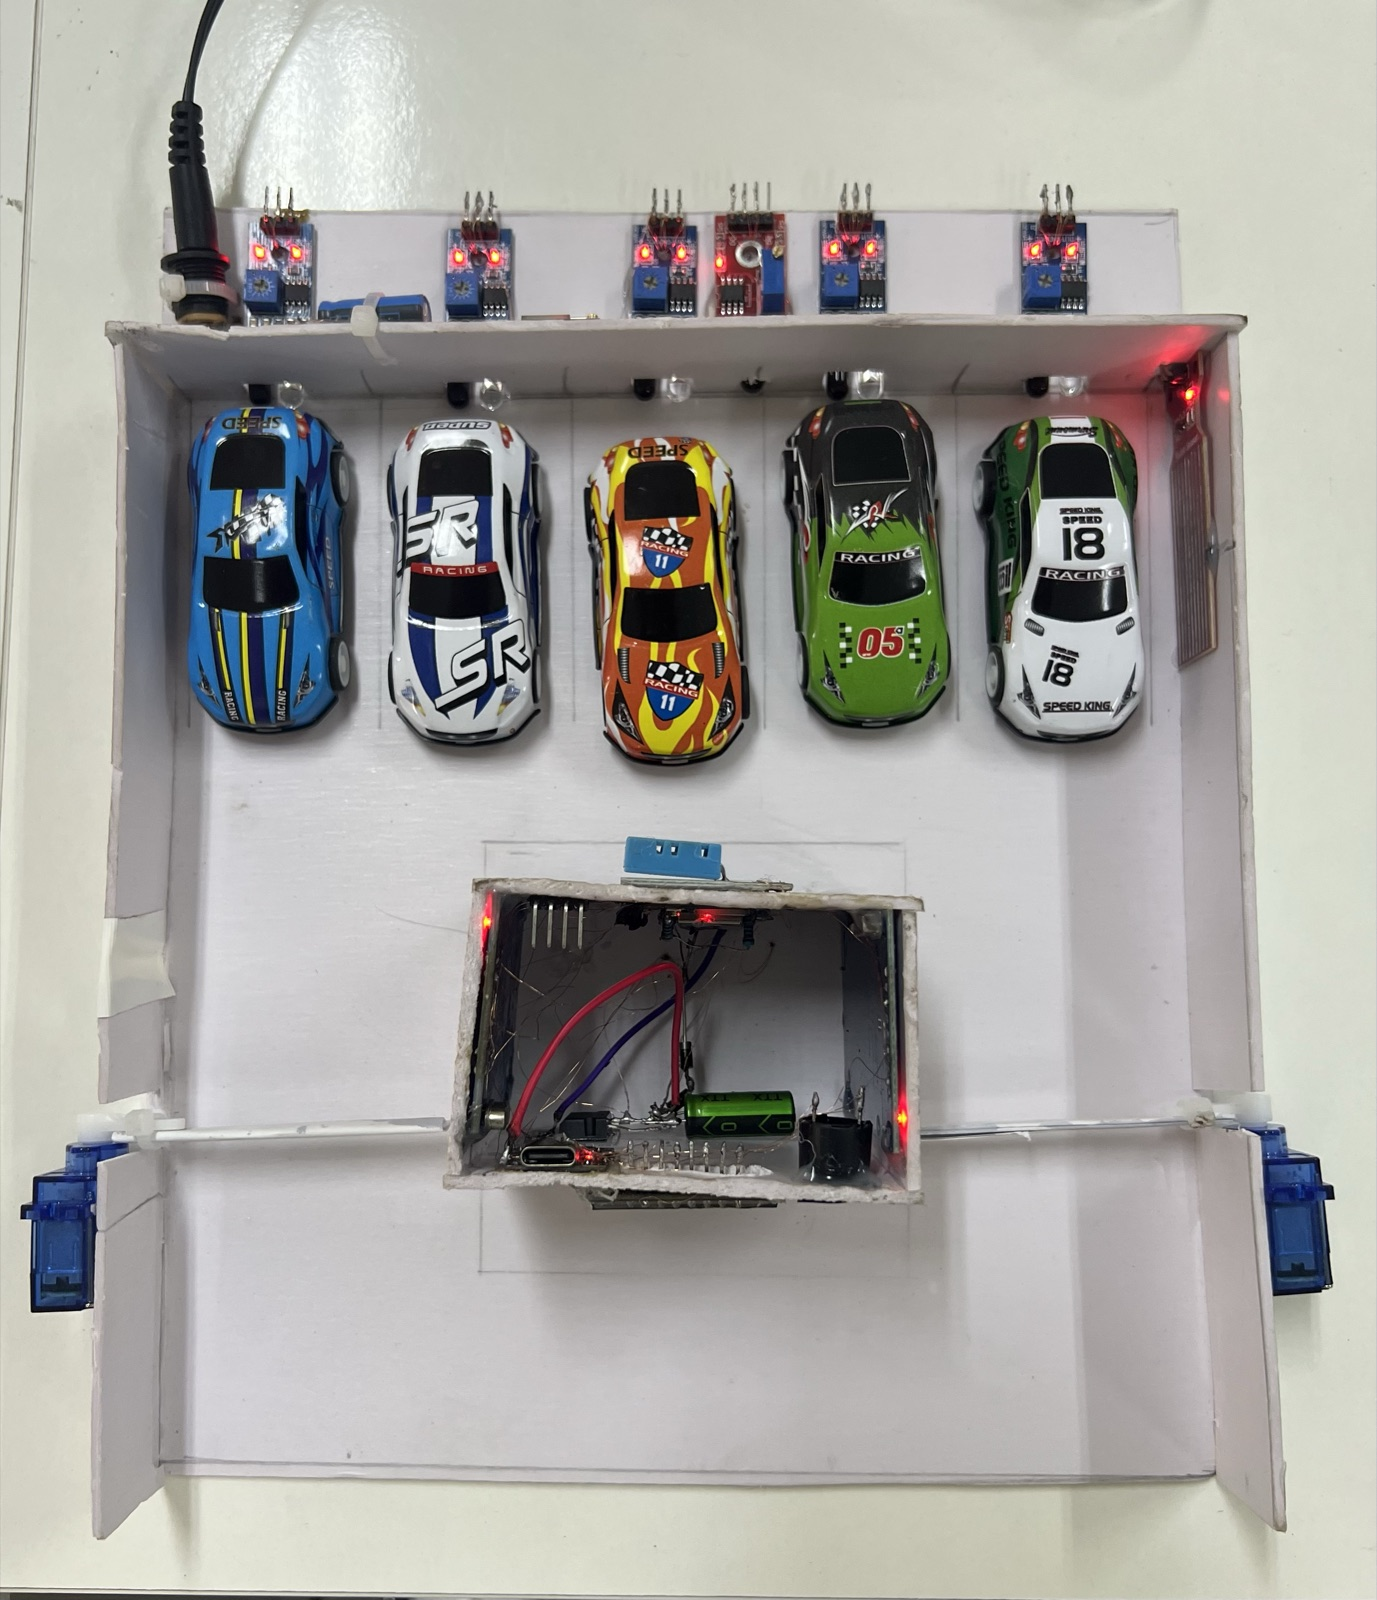
\includegraphics[width=\linewidth,height=0.42\textheight,keepaspectratio]{photos/model_top.jpg}
\caption{Mô hình bãi đỗ xe thông minh nhìn từ trên xuống}\label{fig:overview}
\end{figure}

Từ góc nhìn của người sử dụng, hệ thống vận hành như sau. Khi tới cổng vào, người lái xem
số chỗ trống trên màn hình và quẹt thẻ RFID; thanh chắn tự nâng lên, xe đi qua và thanh
chắn chỉ hạ xuống khi cảm biến ở cổng xác nhận xe đã ra khỏi vùng thanh chắn. Khi xe đỗ vào
một ô, màn hình và trang web quản lý cập nhật trạng thái ô đó trong khoảng một phần mười
giây. Khi ra, người lái quẹt cùng thẻ ở cổng ra; màn hình hiển thị phí gửi xe và một mã
VietQR mà mọi ứng dụng ngân hàng đều quét được. Ngay khi giao dịch chuyển khoản được xác
nhận, thanh chắn cổng ra mở và màn hình hiển thị hóa đơn. Người quản lý theo dõi toàn bộ
bãi, nhật ký xe vào ra và doanh thu trên trang web từ điện thoại mà không cần cài ứng dụng.
Khi xảy ra sự cố, phản ứng của hệ thống phụ thuộc vào loại sự cố: với cháy, còi báo động
được kích hoạt và cả hai thanh chắn được nâng lên để giải phóng lối thoát; với ngập nước, hệ
thống tạm dừng tiếp nhận xe cho tới khi mực nước trở về mức an toàn.

\section{Mục tiêu}
Mục tiêu của đề tài được xác định thành các yêu cầu có thể kiểm chứng trên mô hình. Các mục
tiêu cụ thể gồm:
\begin{itemize}
  \item Xác định trạng thái từng ô đỗ theo thời gian thực, với độ trễ hiển thị tại bãi dưới
        0,2\,s và trên trang web khoảng 1\,s;
  \item Kiểm soát xe ra vào bằng thẻ RFID, từ chối các lần quẹt sai cổng hoặc khi bãi đầy,
        và không hạ thanh chắn khi xe còn nằm trong cổng;
  \item Tính phí tự động theo giờ và thu phí bằng chuyển khoản VietQR với số tiền cố định,
        tự xác nhận giao dịch trước khi mở cổng ra;
  \item Phát hiện cháy và ngập nước, cảnh báo tại chỗ và trên trang web, mở lối thoát khi
        có cháy;
  \item Cho phép người vận hành quản lý bãi và điều khiển thanh chắn từ xa qua trình duyệt, có xác thực
        bằng mã PIN cho các thao tác điều khiển.
\end{itemize}

\section{Khảo sát các giải pháp hiện có}\label{sec:thitruong}
Bãi đỗ xe thông minh không phải là ý tưởng mới. Theo Knowledge Sourcing Intelligence, thị
trường toàn cầu đạt khoảng 8,8 tỷ USD năm 2025 và được dự báo đạt 20,4 tỷ USD năm 2030, trong
đó khu vực châu Á -- Thái Bình Dương tăng trưởng nhanh nhất [16]; Meticulous Research dự báo
quy mô 22,9 tỷ USD vào năm 2032 [17]. Các sản phẩm hiện có có thể chia thành ba nhóm theo
chức năng chính.

Nhóm thứ nhất là phần mềm quản lý bãi giữ xe như eParking, HTG Parking hay Megaparking. Các
phần mềm này ghi nhận lượt xe vào ra, quản lý vé và doanh thu, một số sản phẩm có nhận dạng
biển số hoặc dùng thẻ RFID [22], nhưng không biết xe đang đỗ ở vị trí nào. Nhóm thứ hai là
hệ thống kiểm soát ra vào trọn gói của các nhà tích hợp như KPS System hay Hikvision, gồm
thanh chắn, camera nhận dạng biển số, đầu đọc RFID tầm xa và phần mềm quản lý có kết nối với
hệ thống tòa nhà [18], [19]. Nhóm thứ ba là hệ thống phát hiện xe theo từng chỗ đỗ, tiêu biểu là
cảm biến không dây Nedap SENSIT và hệ thống dẫn hướng của SKIDATA [20], [21], vốn trả lời
câu hỏi chỗ nào còn trống nhưng cần một nền tảng khác để thu phí.

Ở quy mô đô thị, Hà Nội thí điểm ứng dụng iParking từ năm 2017 nhưng dừng chức năng thanh
toán tại 12 đơn vị từ tháng 9/2020, một phần do nhân viên nhập sai số xe khiến doanh thu
không khớp với thực tế [23], [24]. Trong khi đó, thu phí không dừng đang được mở rộng: từ
tháng 5/2024 đã áp dụng tại 5 sân bay lớn [25], và Kế hoạch 198/KH-UBND yêu cầu từ ngày
1/7/2026, toàn bộ bãi đỗ ô tô tại Hà Nội thu giá dịch vụ theo hình thức điện tử không dừng [26].

\begin{table}[H]
\centering\small
\caption{So sánh đề tài với các nhóm giải pháp đã khảo sát}\label{tab:sosanh}
\begin{tabularx}{\linewidth}{@{}>{\raggedright\arraybackslash}p{2.9cm}*{3}{>{\raggedright\arraybackslash}X}@{}}
\toprule
Tiêu chí & Kiểm soát ra vào (KPS, Hikvision) & Cảm biến từng chỗ (Nedap, SKIDATA) & Đề tài \\ \midrule
Nhận dạng xe & Biển số, RFID tầm xa, QR & Không & RFID tầm gần \\
Trạng thái từng chỗ & Không có trong tài liệu & Có, là chức năng chính & Có, 5 cảm biến hồng ngoại \\
Tính phí, thanh toán & Có, nhiều quy tắc giá & Cần hệ thống khác & Tự tính phí, VietQR tự đối soát \\
Cảnh báo cháy, ngập gắn với thanh chắn & Không có trong tài liệu & Không có trong tài liệu & Có, cháy thì mở cả hai cổng \\
Hạ tầng & Máy chủ và phần mềm riêng & Nền tảng quản lý riêng & Chạy trên một vi điều khiển \\
Mức hoàn thiện & Vận hành thực tế nhiều năm & Triển khai quy mô đô thị & Mô hình 5 chỗ, 2 cổng \\
\bottomrule
\end{tabularx}
\end{table}

Bảng~\ref{tab:sosanh} đối chiếu đề tài với hai nhóm giải pháp có chức năng gần nhất. Phân
tích cho thấy ở quy mô lớn, các giải pháp thương mại đã rất hoàn thiện về nhận dạng xe, tốc
độ qua cổng và khả năng tích hợp; đề tài không nhằm cạnh tranh ở quy mô đó. Khoảng trống
nằm ở các bãi nhỏ: phát hiện chỗ trống, kiểm soát ra vào, thanh toán và cảnh báo an toàn thường
thuộc những sản phẩm riêng biệt, phải qua nhà tích hợp và không có giá niêm yết [27]. Bài
học từ iParking cũng cho thấy việc phụ thuộc vào người nhập liệu là nguồn sai lệch doanh thu.
Đề tài hướng tới khoảng trống này với ba đặc điểm: gộp đủ các chức năng trong một hệ thống
chi phí thấp, tính phí và đối soát giao dịch hoàn toàn tự động, và gắn cảnh báo an toàn
trực tiếp với cơ cấu thanh chắn. Đổi lại, hệ thống chưa có nhận dạng biển số và đầu đọc tầm
xa, nên xe vẫn phải dừng để quẹt thẻ.
